% METODOLOGIA------------------------------------------------------------------

\chapter{MATERIAL E MÉTODOS}
\label{chap:metodologia}

O objetivo deste trabalho é propor um método para implementação de testes automatizados em conjunto a métodos ágeis no projetos de software. Buscando atingir tal objetivo o desenvolvimento do trabalho consistiu de algumas etapas (\autoref{fig:bpmn-metodos-tcc}):

    \begin{figure}[!htb]
        \centering
    	\sbox0{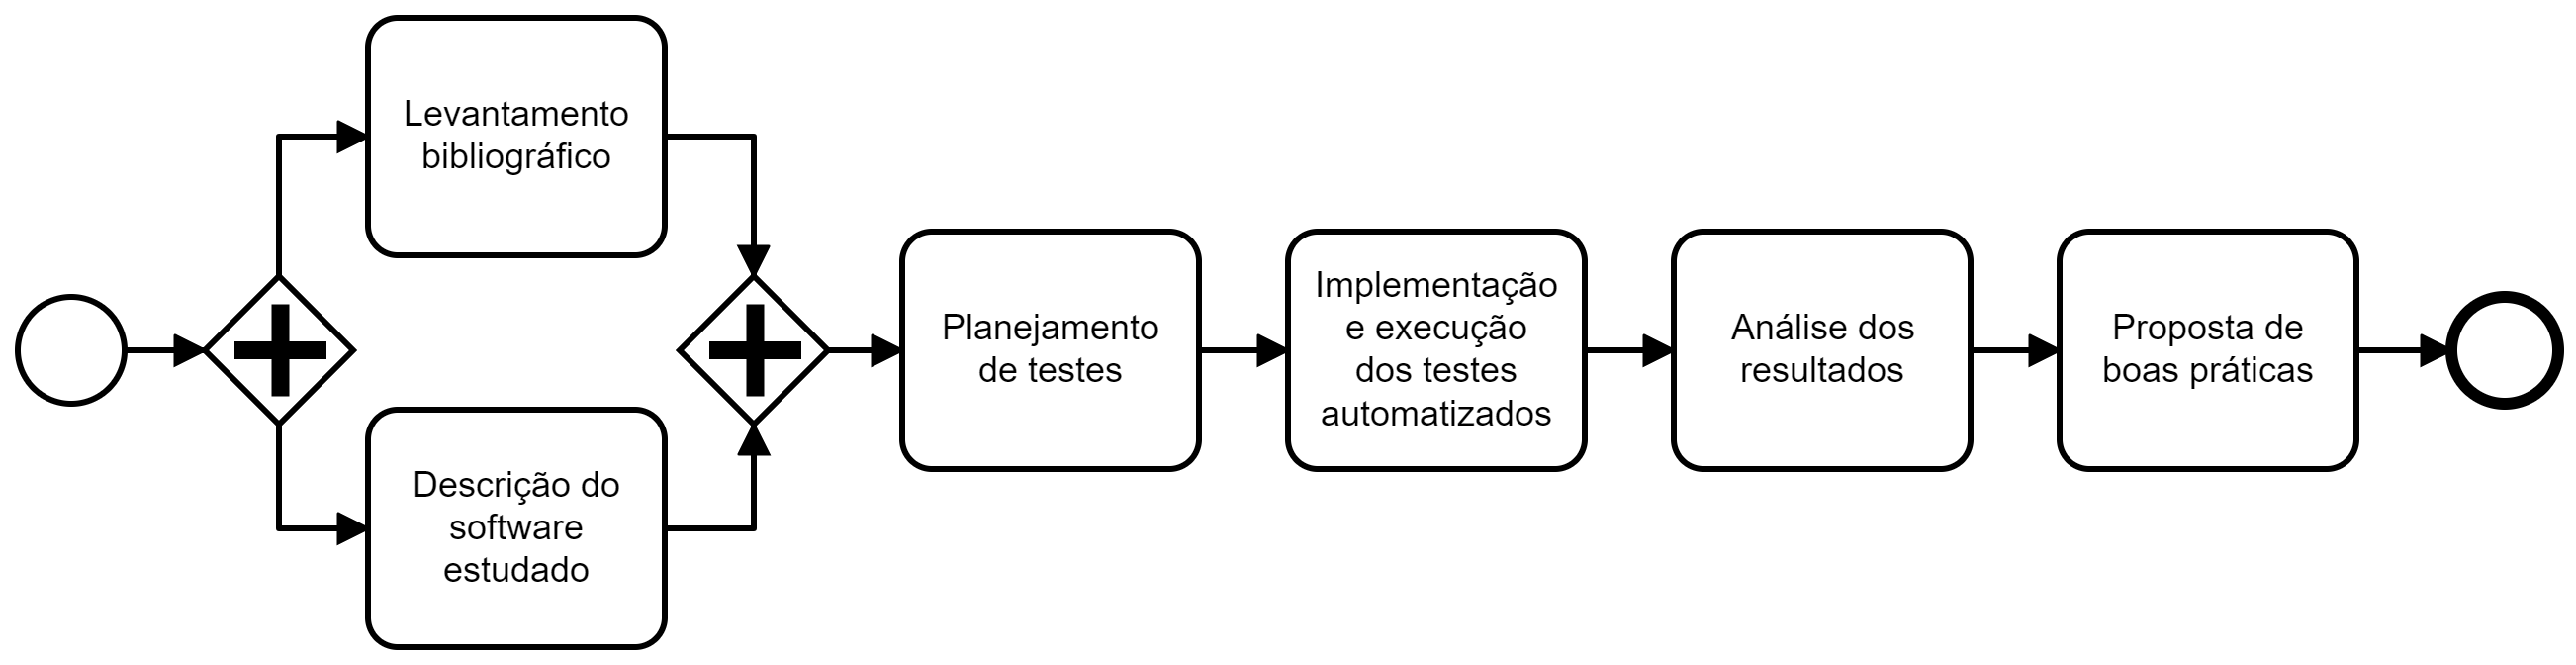
\includegraphics[width=1\textwidth]{./assets/figuras/bpmn_metodos_tcc}}% measure width
    	\begin{minipage}{\wd0}
	    	\usebox0
	    	\caption{Desenvolvimento do Trabalho}
	    	\label{fig:bpmn-metodos-tcc}
		    \fonte{o Autor}
	    \end{minipage}
    \end{figure}

   \section{DESCRIÇÃO DO SOFTWARE ESTUDADO}
    O conjunto de práticas de teste de software que pode ser aplicado em um software depende do contexto, ou seja, dependendo do processo, do projeto ou mesmo do software que é testado, algumas práticas podem ser mais apropriadas que outras. A fim de explorar a aplicação das práticas apropriadas, será realizado um estudo de caso da aplicação das práticas de teste de software nas atividades de teste do Sistema Admink.

    O Sistema Admink consiste em uma aplicação web, ou seja, um sistema de informação projetado para ser utilizado através de navegadores na internet, que foi desenvolvido há alguns meses pelo autor desta monografia e pelo estudante Thiago Teixeira durante a disciplina de Projeto do curso de Engenharia de Software da Universidade Estadual de Ponta Grossa.

    O Admink foi projetado para apoiar a administração de estúdios de tatuagem através do gerenciamento de informações importantes para o dia a dia do estúdio como dados de clientes, tatuadores, orçamentos, espaços de trabalho, agendamentos de tatuagem e indicadores de apoio à gestão. Previamente ao desenvolvimento do Sistema Admink foram produzidos documentos de casos de uso (\autoref{chap:apendiceA}) e casos de teste (\autoref{chap:apendiceB}).

    O Sistema Admink foi desenvolvido utilizando a linguagem de programação \emph{PHP} na versão 7.3.33, o \emph{framework PHP Laravel} na versão 6.20.44, e o sistema gerenciador de banco de dados relacionais de código aberto MariaDB na versão 10.4.13. O código do sistema está armazenado e versionado em um repositório no \emph{GitHub}.

    \emph{PHP} é uma linguagem de programação interpretada é direcionada para desenvolvimento para a \emph{web} com o principal objetivo de permitir a criação de páginas geradas dinamicamente rapidamente \cite{PHP2021}.

    \emph{Laravel} é um \emph{framework} para aplicações \emph{web} com sintaxe elegante e expressiva. Um \emph{framework} para aplicações \emph{web} fornece a estrutura e ponto inicial para criação das aplicações, permitindo que desenvolvedores foquem na criação da aplicação sem se preocupar com todos os detalhes. O \emph{Laravel} fornece recursos para a criação, configuração e execução de testes unitários e de integração, pois adota por padrão o \emph{PHPUnit}, que é um \emph{framework} de testes unitários para PHP \cite{Laravel2021}.

    O \emph{PHPUnit} é um um \emph{framework} de testes orientado ao programador, baseado na arquitetura \emph{xUnit} para \emph{frameworks de testes de unidade}, suportando a realização de testes automatizados. Assim como outros \emph{frameworks} de testes de unidade, o \emph{PHPUnit} utiliza asserções (\emph{assertions}) para verificar a conformidade do comportamento apresentado pelo código-fonte com o comportamento esperado. As asserções são métodos criados para garantir que o valor recebido em um teste é o valor esperado e no \emph{PHPUnit} há pelo menos 46 métodos de asserção disponíveis \cite{PHPcombr}.
    
    O Sistema Admink também conta com \emph{factories} que foram criadas durante a implementação para apoiar o desenvolvimento e a realização dos testes. As \emph{Factories} permitem que um conjunto de atributos seja definido para popular no banco de dados as tabelas de entidades que possuem classes equivalentes no código da aplicação. Quando utilizadas em conjunto com \emph{faker} o conjunto de dados pode ser gerado com valores aleatórios \cite{Laravel2021}.

    O \emph{GitHub} fornece serviços de hospedagem de repositórios baseados em nuvem, permitindo controle de versão e colaboração de forma remota.
   
    \section{LEVANTAMENTO BIBLIOGRÁFICO}

        Nesta etapa foi realizado o levantamento bibliográfico para auxílio na implementação dos testes e do entendimento do fluxo de trabalho proposto por métodos ágeis. A partir dos trabalhos encontrados descreveu-se a relação das atividades de teste de software com os processos de desenvolvimento de software e a evolução de ambos com o passar dos anos. Também foram descritas as atividades de teste de software e de testes automatizados, incluindo as técnicas utilizadas para identificação dos testes necessários para verificar aplicações de forma eficaz.

        Após entender quão amplos são os estudos de teste de software e mesmo de testes automatizados, manifestou-se a necessidade de delimitar um escopo específico como foco deste trabalho. Optou-se por estudar a implementação de testes funcionais em um dos níveis de teste automatizado para dois casos de uso do Sistema Admink. Foram escolhidos o nível de teste de integração e os casos de uso \textbf{Efetuar Login} e \textbf{Manter Orçamentos} para serem estudados neste trabalho.

    \section{PLANEJAMENTO DE TESTES}
        
        Na etapa de Planejamento de Testes foi realizada a análise de parte da documentação previamente criada do Sistema Admink, além da utilização de técnicas de teste de caixa preta para identificação dos cenários de testes. Em seguida os cenários de testes identificados foram representados em diagramas baseados em mapas mentais.

        \subsection{Representação dos cenários de teste baseada em mapas mentais}
 
            Buscando atender às necessidades de equipes que aplicam métodos ágeis com menor foco em documentações detalhadas, evitou-se a utilização de documentos extensos e que necessitem de muito tempo para serem interpretados para representação dos cenários de teste, então, propôs-se um método de representação de cenários de teste utilizando diagramas baseados em mapas mentais, contendo as principais informações necessárias para apoiar a implementação dos \emph{scripts} de testes automatizados.
            
            Mapas mentais são um método de representar informações de forma organizada e priorizada, baseado no uso de palavras-chave e imagens-chave capazes de resgatar memórias específicas, além de estimular novos pensamentos \cite{Buzan2009}.
 
            Para criação dos diagramas baseados em mapas mentais foi utilizada a aplicação web \emph{XMind}, ferramenta destinada para criação de mapas mentais e realização de \emph{brainstorm} \cite{XMind2022}. Entretanto, outras aplicações ou ferramentas voltadas para criação de diagramas baseados em mapas mentais também poderiam ser utilizadas sem prejuízos à aplicação do método. O método proposto consiste nos seguintes passos (\autoref{fig:template-mind-map-tcc}):
            
            \begin{figure}[!htb]
                \centering
	            \sbox0{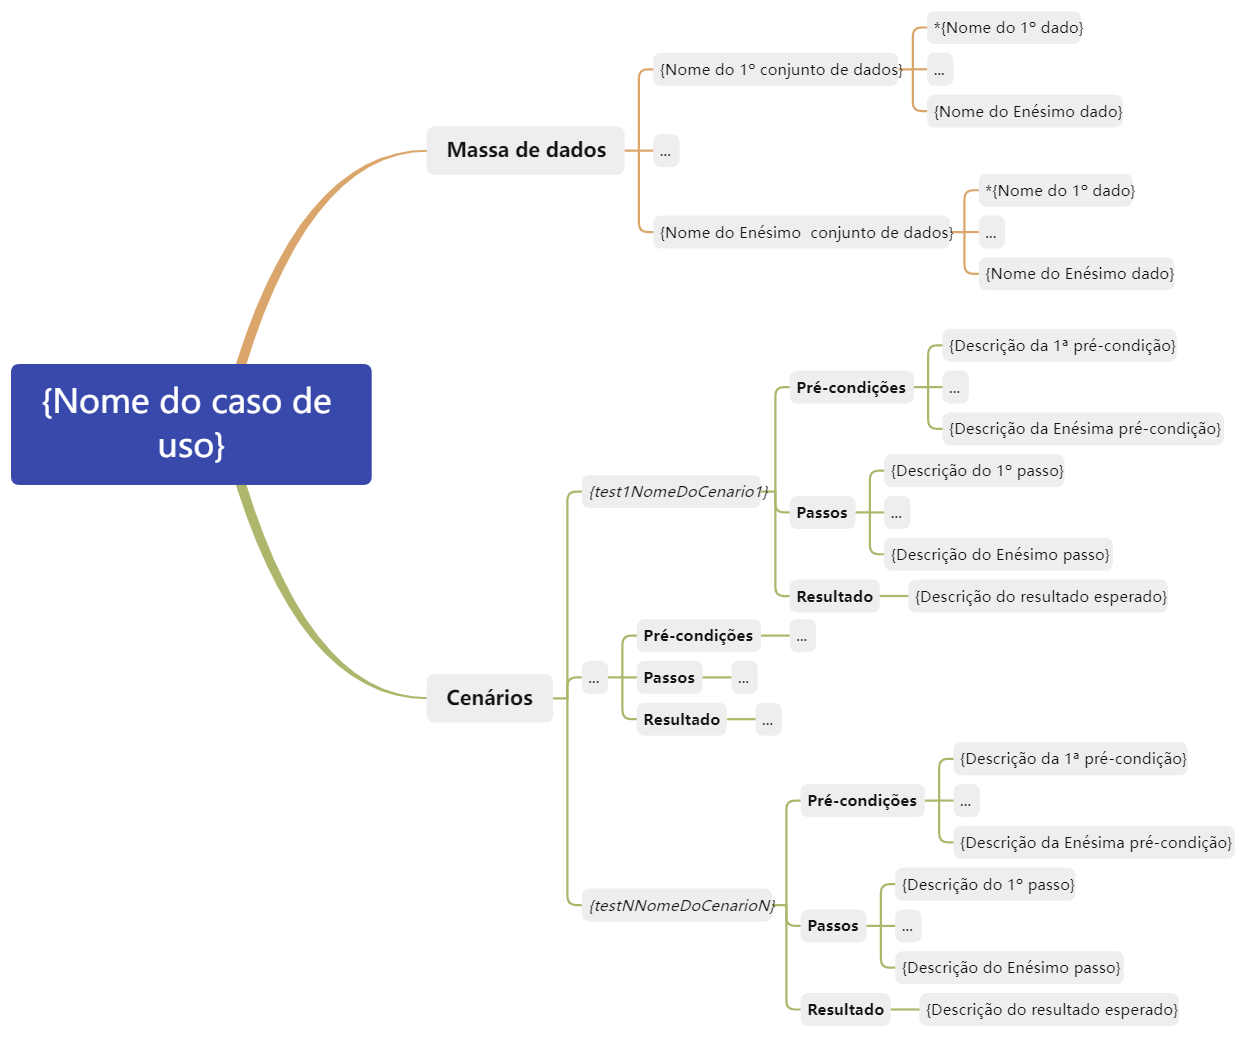
\includegraphics[width=1\textwidth]{./assets/figuras/testing_mind_map_template}}% measure width
	            \begin{minipage}{\wd0}
		            \usebox0
		            \caption{ Esquema representando o diagrama proposto pelo método para representação de cenário de testes utilizando diagramas baseados em mapas mentais onde cada um dos itens delimitados por chaves podem ser editados conforme as informações correspondente dos cenários de teste e os itens exibidos em negrito são fixos e não são editados independente das informações dos cenários de teste
		            }  
		            \label{fig:template-mind-map-tcc}
		            \fonte{o Autor}
	            \end{minipage}
            \end{figure}

            \begin{itemize}
                \item Inicia-se o digrama preenchendo a informação central do diagrama com o nome do caso de uso, história de usuário ou funcionalidade para a qual os cenários de teste serão representados;
                \item Em seguida são criados os ramos \textbf{Cenários} e \textbf{Massa de dados};
                \item A seguir são inseridos novos ramos ligados diretamente aos ramos \textbf{Cenários} e \textbf{Massa de dados}, os quais são preenchidos com as informações de cenários de testes de integração e os dados necessários para realização dos testes, respectivamente. Buscando facilitar a identificação de qual parte do código de \emph{scripts} de testes de integração corresponde a cada um dos cenários mapeados, utilizou-se a mesma nomenclatura para os ramos que representam os cenários e para o título dos métodos de teste nos \emph{scripts};
                \item Em cada um dos ramos de cenários criados são adicionados os ramos \textbf{Passos} e \textbf{Resultados}. No ramo \textbf{Passos} são descritos os passos que devem ser executados durante a realização do teste. No ramo \textbf{Resultados} é descrito o resultado que é esperado que a aplicação apresente após a execução dos passos descritos no ramo \textbf{Passos}.
            \end{itemize}
        
            Após definido o método de representação, os cenários de teste planejados para os casos de uso \textbf{Efetuar Login} e \textbf{Manter Orçamentos} foram representados utilizando o método de representação proposto. Os cenários de teste para o caso de uso \textbf{Efetuar Login} foram representandos em um único diagrama, entretanto para o caso de uso \textbf{Manter Orçamentos} foi criado um diagrama para cada funcionalidade, buscando facilitar a visualização e evitando um diagrama muito extenso.
            
    \section{IMPLEMENTAÇÃO E EXECUÇÃO DOS TESTES AUTOMATIZADOS}
        A partir da delimitação do escopo deste trabalho, consultou-se a seção \emph{Testing} da documentação da versão do \emph{Framework Laravel} utilizada no desenvolvimento do Sistema Admink a fim de descobrir as recomendações para realização de testes de integração. Descobriu-se que projetos criados a partir do \emph{Framework Laravel} já são pré-configurados por padrão com os recursos para criação de testes unitários e de integração, utilizando \emph{PHPUnit}, e que é recomendado utilizar esses recursos para a criação dos \emph{scripts} de testes automatizados.
 
        Após os cenários de testes estarem representados nos diagramas baseados em mapas mentais, iniciou-se a codificação dos \emph{scripts} de testes de integração automatizados utilizando os diagramas como base e seguindo as instruções da documentação do \emph{Framework Laravel} e do \emph{PHPUnit}. Além dos diagramas, o código foi analisado para entender como a aplicação está estruturada e quais partes do código deveriam ser utilizadas para realização dos testes.
        
        Baseando-se nas informações fornecidas pelos diagramas cada um dos \emph{scripts} de teste foi criado utilizando o framework para testes de unidade emph{PHPUnit} na versão 9.5.17. Cada um dos itens de cada diagrama foi analisado para criar os \emph{scripts} de teste:
        
        \begin{itemize}
            \item Inicialmente foi criada uma classe por digrama para conter os métodos referentes aos cenários de teste representados em cada diagrama;
            \item Em seguida analisou-se as informações presentes nos itens referentes a \textbf{Massa de dados} para identificar os dados necessários para realização dos testes e como prepará-los para serem utilizados nos \emph{scripts};
            \item A partir dos itens referentes aos \textbf{Cenários} são criados métodos de teste com os mesmos nomes mostrados nos diagramas;
            \item A partir dos itens referentes às \textbf{Pré-condições} são implementados nos métodos de teste as ações que devem ser realizadas antes dos passos de cada teste;
            \item A partir dos itens referentes aos \textbf{Passos} são implementadas nos métodos as ações que que devem causar os resultados esperados na aplicação;
            \item Por fim, as asserções são criadas nos métodos de teste esperando como retorno da aplicação as mesmas informações presentes nos itens referentes ao \textbf{Resultado} de cada cenário de teste presente no diagrama.
        \end{itemize}
        
        Após criados os \emph{scripts} de teste foi realizada a execução dos mesmos em um computador equipado com o Sistema Operacional Windows 10 Pro na versão 21H1, com processador Intel(R) Core(TM) i5-10210U de 1.60GHz, com 16 GB de memória principal e com uma unidade de estado sólido de 256 GB. Foram realizados 30 execuções sucessivas dos \emph{scripts} de teste criados e coletados os dados de tempo de execução para calcular-se o tempo médio gasto nessas execuções.
        
        Os resultados obtidos após a realização dos métodos e experimentos acima descritos serão explorados no \autoref{chap:resultados}. 